\documentclass[11pt]{article}
\usepackage[a4paper,margin=2.2cm]{geometry}
\usepackage[T1]{fontenc}
\usepackage[utf8]{inputenc}
\usepackage{lmodern}
\usepackage{microtype}
\usepackage{booktabs}
\usepackage{tabularx}
\usepackage{array}
\usepackage{enumitem}
\usepackage{xcolor}
\usepackage{listings}
\usepackage[most]{tcolorbox}
\usepackage{tikz}
\usetikzlibrary{arrows.meta,positioning,fit,backgrounds}
\usepackage[colorlinks=true,linkcolor=blue!50!black,urlcolor=blue!50!black]{hyperref}
\usepackage{fancyhdr}
\usepackage{needspace}

\setlist{nosep,leftmargin=*,topsep=2pt}
\setlength{\parindent}{0pt}
\setlength{\parskip}{5pt}
\renewcommand{\arraystretch}{1.25}

\definecolor{ink}{HTML}{1D1D1B}
\definecolor{accent}{HTML}{1F4E79}
\definecolor{codebg}{HTML}{F2F1EC}
\definecolor{notebg}{HTML}{EAF1F8}
\definecolor{warnbg}{HTML}{FDF3E1}
\definecolor{okbg}{HTML}{EAF4EA}

\pagestyle{fancy}
\fancyhf{}
\fancyhead[L]{\small\color{gray}ScholarLens user guide}
\fancyhead[R]{\small\color{gray}github.com/madhureddy25/ScholarLens}
\fancyfoot[C]{\small\thepage}
\renewcommand{\headrulewidth}{0.3pt}

\lstset{basicstyle=\ttfamily\small,columns=fullflexible,keepspaces=true,breaklines=true,
        breakatwhitespace=false,upquote=true,showstringspaces=false}
\newtcblisting{cmd}{listing only,colback=codebg,colframe=codebg,boxrule=0pt,arc=2pt,
  left=6pt,right=6pt,top=3pt,bottom=3pt,listing options={basicstyle=\ttfamily\footnotesize,breaklines=true,columns=fullflexible,keepspaces=true}}
\newtcolorbox{note}[1][]{colback=notebg,colframe=notebg,boxrule=0pt,arc=2pt,left=6pt,right=6pt,top=4pt,bottom=4pt,#1}
\newtcolorbox{warn}[1][]{colback=warnbg,colframe=warnbg,boxrule=0pt,arc=2pt,left=6pt,right=6pt,top=4pt,bottom=4pt,#1}
\newtcolorbox{good}[1][]{colback=okbg,colframe=okbg,boxrule=0pt,arc=2pt,left=6pt,right=6pt,top=4pt,bottom=4pt,#1}

\usepackage{titlesec}
\titleformat{\section}{\Large\bfseries\color{accent}}{\thesection}{0.6em}{}
\titleformat{\subsection}{\large\bfseries\color{ink}}{\thesubsection}{0.5em}{}
\titlespacing*{\section}{0pt}{14pt}{6pt}
\titlespacing*{\subsection}{0pt}{10pt}{4pt}

\newcommand{\cm}[1]{\texttt{#1}}

\begin{document}

%-------------------------------------------------------------------- cover
\thispagestyle{empty}
\vspace*{2.5cm}
{\color{accent}\fontsize{34}{40}\selectfont\bfseries ScholarLens}\\[6pt]
{\Large User guide: what it is, how it works, and how to use it}\\[18pt]
{\large Integrity-first tools for academic writing:\\
detect machine-generated text fairly, and edit your own paper without breaking citations.}

\vspace{1.2cm}
\begin{note}
\textbf{Who this is for.} Anyone who wants to use ScholarLens on a paper, or rerun and extend the research.
Every command in this guide is for \textbf{Windows PowerShell} on the project laptop, and was checked against the code.
For the original setup and the full study, see \cm{docs/LAPTOP\_COMMANDS.pdf}.
\end{note}

\vspace{0.6cm}
{\large\bfseries\color{accent} Contents}\\[4pt]
\begin{tabular}{@{}rl@{}}
1 & ScholarLens in one page \\
2 & How the parts fit together \\
3 & Before you start: every PowerShell window \\
4 & Quill: edit your own paper safely (step by step) \\
5 & Lens: check a text for machine-generated prose (step by step) \\
6 & How it works inside \\
7 & Keeping the models improving \\
8 & Rebuilding or extending the research \\
9 & What we found \\
10 & Other tools: inspecting a document, the HTTP API \\
11 & Where everything is \\
12 & Troubleshooting \\
13 & Glossary \\
\end{tabular}

\vfill
{\small\color{gray} Project: \url{https://github.com/madhureddy25/ScholarLens}\quad·\quad Releases: \cm{bench-v1}, \cm{lens-v1}\quad·\quad Guide version: November 2026}
\newpage

%-------------------------------------------------------------------- 1
\needspace{8\baselineskip}\section{ScholarLens in one page}

ScholarLens is a set of command-line tools, written in Python, for two related jobs in academic writing:

\begin{enumerate}
  \item \textbf{Checking} whether a text looks machine-generated, in a way that still works when the text has been paraphrased, and that does not punish honest authors who polished their own writing.
  \item \textbf{Editing} your own draft with an AI model \emph{safely}: citations, equations, numbers and references can never be changed, and every change is shown to you for approval.
\end{enumerate}

It has three main parts plus a learning loop:

\begin{tabularx}{\linewidth}{@{}>{\bfseries}l X X@{}}
\toprule
Part & What it is & What you get from it \\
\midrule
Quill & A citation-safe \textbf{editor} for your own paper (LaTeX, Markdown, Word, plain text). & An edited copy, a tracked-changes copy, a review page, and an AI-use disclosure record. \\
Lens & An \textbf{AI-text detector} trained to resist paraphrasing and checked for false alarms on edited human text. & A score, P(AI), for each section of about 250 words. \\
Bench & The \textbf{benchmark}: 5,500 labelled texts (human, machine, paraphrased machine, edited human). & The data that trains and fairly tests Lens. Published as \cm{bench-v1}. \\
Learning loop & GitHub automation that \textbf{retrains} Lens weekly, and tools to retrain Quill. & New versions published only if they beat the old ones. \\
\bottomrule
\end{tabularx}

\begin{warn}
\textbf{What ScholarLens is \emph{not}.}
\begin{itemize}
  \item \textbf{It is not a ``humanizer''.} Quill never sees a detector score and is never trained to fool detectors. That was a deliberate design decision.
  \item \textbf{A Lens score is not proof.} It is evidence about a text, never a verdict about a person. Never accuse anyone on the basis of a detector score alone.
\end{itemize}
\end{warn}

%-------------------------------------------------------------------- 2
\needspace{8\baselineskip}\section{How the parts fit together}

\begin{center}
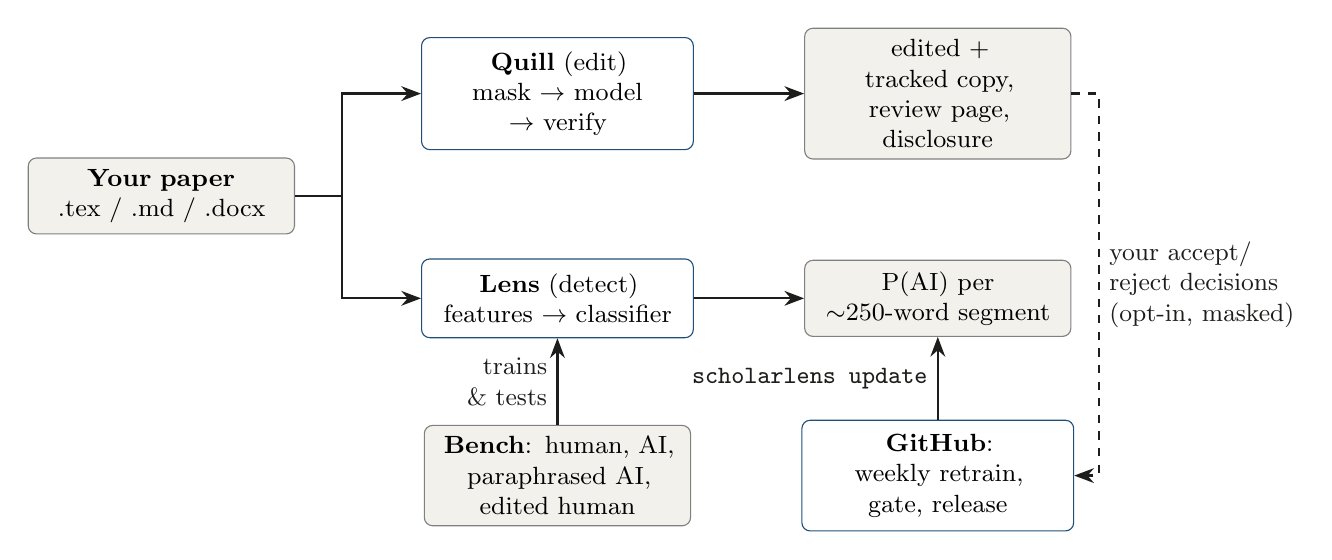
\begin{tikzpicture}[font=\small,
  box/.style={draw=accent,fill=white,rounded corners=3pt,align=center,inner sep=5pt,minimum height=1cm,text width=3.1cm},
  data/.style={draw=gray,fill=codebg,rounded corners=3pt,align=center,inner sep=4pt,minimum height=0.9cm,text width=3.1cm},
  arr/.style={-{Stealth[length=2.5mm]},thick,color=ink}]
\node[data] (paper) {\textbf{Your paper}\\ .tex / .md / .docx};
\node[box, right=1.6cm of paper, yshift=1.3cm] (quill) {\textbf{Quill} (edit)\\ mask $\rightarrow$ model $\rightarrow$ verify};
\node[box, right=1.6cm of paper, yshift=-1.3cm] (lens) {\textbf{Lens} (detect)\\ features $\rightarrow$ classifier};
\node[data, right=1.4cm of quill] (qout) {edited + tracked copy,\\ review page, disclosure};
\node[data, right=1.4cm of lens] (lout) {P(AI) per\\ $\sim$250-word segment};
\node[data, below=1.1cm of lens] (bench) {\textbf{Bench}: human, AI,\\ paraphrased AI, edited human};
\node[box, right=1.4cm of bench] (gh) {\textbf{GitHub}: weekly retrain,\\ gate, release};
\draw[arr] (paper.east) -- ++(0.6,0) |- (quill.west);
\draw[arr] (paper.east) -- ++(0.6,0) |- (lens.west);
\draw[arr] (quill) -- (qout);
\draw[arr] (lens) -- (lout);
\draw[arr] (bench) -- node[left,align=right]{trains\\ \& tests} (lens);
\draw[arr] (gh.north) -- node[left]{\cm{scholarlens update}} (lout.south);
\draw[arr,dashed] (qout.east) -- ++(0.35,0) |- node[pos=0.25,right,align=left]{your accept/\\reject decisions\\(opt-in, masked)} (gh.east);
\end{tikzpicture}
\end{center}

\textbf{In words:}
\begin{itemize}
  \item \textbf{Quill} takes your paper, hides everything that must not change, asks a language model to improve only the prose, checks the result, and shows you the changes.
  \item \textbf{Lens} reads a text and estimates how likely each part is to be machine-generated.
  \item \textbf{Bench} is the data Lens learned from and is tested on.
  \item \textbf{GitHub} retrains Lens every week and publishes a new version only if it is better on a frozen test set. Your decisions in Quill can help improve the models, but only if you choose to share them.
\end{itemize}

%-------------------------------------------------------------------- 3
\needspace{8\baselineskip}\section{Before you start: every PowerShell window}

Open \textbf{PowerShell} and run these two commands first, every time:
\begin{cmd}
cd $HOME\ScholarLens
.\.venv\Scripts\Activate.ps1
\end{cmd}
The prompt should start with \cm{(.venv)}. In this guide, a line ending in a backtick (\cm{`}) continues on the next line: copy the whole grey block and paste it at once.

To check that everything is ready:
\begin{cmd}
scholarlens --help
python -c "import torch; print(torch.__version__, torch.cuda.is_available())"
\end{cmd}
The second command should print \cm{...+cu126 True}, which means the GPU is in use. If it prints \cm{False}, see Troubleshooting (\S\ref{sec:trouble}).

To get the newest code and models:
\begin{cmd}
git pull
scholarlens update lens
\end{cmd}

%-------------------------------------------------------------------- 4
\needspace{8\baselineskip}\section{Quill: edit your own paper safely}

\needspace{5\baselineskip}\subsection*{Step 1. Make sure a model is available}
Quill needs a language model to do the editing. The easiest choice runs on your laptop for free through Ollama.
The Ollama app must be running (Start menu, then Ollama):
\begin{cmd}
ollama list
\end{cmd}
You should see \cm{qwen2.5:7b}. If not: \cm{ollama pull qwen2.5:7b}.

\needspace{5\baselineskip}\subsection*{Step 2. Run Quill on your paper}
\begin{cmd}
scholarlens edit mypaper.tex -m ollama:qwen2.5:7b --mode proofread
\end{cmd}
Replace \cm{mypaper.tex} with your file. Word (\cm{.docx}), Markdown (\cm{.md}) and plain text (\cm{.txt}) work too.
Quill prints one line per paragraph:

\begin{tabularx}{\linewidth}{@{}>{\ttfamily}l X@{}}
\toprule
\normalfont Status & Meaning \\
\midrule
accepted & An improved version passed all checks and is proposed to you. \\
unchanged & The model found nothing to change. \\
rejected & The model broke something (e.g. dropped a citation); the original is kept. This is the safety net working. \\
skipped & Too short to edit (headings, captions). \\
\bottomrule
\end{tabularx}

\needspace{5\baselineskip}\subsection*{Step 3. Look at the changes}
Quill writes a folder next to your file, e.g. \cm{mypaper\_quill\textbackslash}:

\begin{tabularx}{\linewidth}{@{}>{\ttfamily}l X@{}}
\toprule
\normalfont File & What it is \\
\midrule
mypaper.review.html & \textbf{Open this in your browser}: every change side by side. \\
mypaper.tracked.tex & Your paper with changes marked (for .docx: real Word tracked changes). \\
mypaper.edited.tex & Your paper with all proposed changes applied. \\
mypaper.disclosure.json & Record of which model edited what: use it for an AI-use statement. \\
mypaper.session.json & Needed for Step 4. \\
\bottomrule
\end{tabularx}

\needspace{5\baselineskip}\subsection*{Step 4. Accept or reject each change}
\begin{cmd}
scholarlens review mypaper_quill\mypaper.session.json
\end{cmd}
It asks about each edit. To accept everything without asking, add \cm{-{}-accept-all}. The final paper is written with \textbf{only the edits you accepted}.

\needspace{5\baselineskip}\subsection*{Choosing a mode and a model}
\begin{tabularx}{\linewidth}{@{}>{\ttfamily}l X@{}}
\toprule
\normalfont \texttt{-{}-mode} & What it changes \\
\midrule
proofread & Grammar, spelling, punctuation only. Smallest changes. \\
clarity & Light rewording for readability (the default). \\
concise & Shortens wordy sentences. \\
\bottomrule
\end{tabularx}

\begin{tabularx}{\linewidth}{@{}>{\ttfamily}l X@{}}
\toprule
\normalfont \texttt{-m} (model) & Notes \\
\midrule
ollama:qwen2.5:7b & \textbf{Recommended.} Free, local, good quality on the 6\,GB GPU. \\
quill:models/quill-rl-v1 & Our RL-trained 0.5B editor. Very safe but makes very few changes (\S\ref{sec:results}). \\
anthropic:<model> & A hosted Claude model; needs an API key (\cm{ANTHROPIC\_API\_KEY}). Your paragraphs are sent to the provider, with protected content masked. \\
hf:<model> & Any Hugging Face model run locally. \\
\bottomrule
\end{tabularx}
\smallskip
\cm{scholarlens models} lists every provider and profile.

\needspace{5\baselineskip}\subsection*{Useful options}
\begin{itemize}
  \item \cm{-{}-sections "Introduction,Related Work"}: edit only these sections.
  \item \cm{-{}-glossary terms.txt}: extra words that must never change, one per line.
  \item \cm{-{}-dry-run}: show exactly what would be sent to the model, without calling it.
  \item \cm{-{}-min-similarity 0.94}: how close in meaning an edit must stay. Higher is stricter.
\end{itemize}

\begin{good}
\textbf{What Quill always protects:} citations (\cm{\textbackslash cite\{\}}), references (\cm{\textbackslash ref\{\}}), equations and maths, numbers and statistics, URLs, LaTeX commands, and domain terms (gene names, acronyms, formulas, your glossary).
Only prose paragraphs are ever changed; every other byte of your file stays identical.
\end{good}

%-------------------------------------------------------------------- 5
\needspace{8\baselineskip}\section{Lens: check a text for machine-generated prose}

\needspace{5\baselineskip}\subsection*{Step 1. Install the current detector (once, then occasionally)}
\begin{cmd}
scholarlens update lens
\end{cmd}
This downloads the newest published Lens (currently \cm{lens-v1}) and verifies its checksum.

\needspace{5\baselineskip}\subsection*{Step 2. Score a document}
\begin{cmd}
scholarlens detect mypaper.tex
\end{cmd}
To use a model you trained yourself instead: \cm{-{}-model models\textbackslash lens-v1}.

\needspace{5\baselineskip}\subsection*{Step 3. Read the result}
Lens splits the prose into segments of about 250 words and prints a table:
\cm{segment}, the paragraphs it covers (\cm{nodes}), \cm{words}, and \cm{P(AI)}: the estimated probability, from 0 to 1, that the segment is machine-generated.

\begin{warn}
\textbf{How to interpret P(AI) responsibly:}
\begin{itemize}
  \item \textbf{It is a probability for a text, not a judgement of a person.} Treat high values as a reason to look closer, never as proof.
  \item \textbf{Lens was trained and tested on arXiv-style abstracts} (mostly physics). Full papers, other fields and other genres may score differently.
  \item \textbf{At our strict setting} (1 false alarm per 100 human abstracts), Lens catches about 88\% of plain machine abstracts but only about half of heavily paraphrased ones. A low score does not prove human authorship either.
  \item \textbf{Light, honest editing} (proofreading, clarity) raised false alarms only slightly in our tests (1 in 46). Heavier rewriting and non-native authors were \emph{not} tested yet.
\end{itemize}
\end{warn}

%-------------------------------------------------------------------- 6
\needspace{8\baselineskip}\section{How it works inside}

\subsection{Quill: the editing pipeline}
\begin{enumerate}
  \item \textbf{Parse.} The file is split into nodes (paragraphs, headings, equations, commands). Only prose nodes can be edited.
  \item \textbf{Mask.} Inside each paragraph, protected content is replaced by placeholders such as \cm{[[CITE\_1]]} or \cm{[[MATH\_2]]} (Quill uses special bracket characters).
  \item \textbf{Ask the model} to edit the masked paragraph in the chosen mode.
  \item \textbf{Verify.} Every placeholder must come back exactly once, LaTeX braces must balance, and the meaning must stay close: semantic similarity of at least 0.94, measured with a sentence-embedding model.
  \item \textbf{Retry or keep the original.} If a check fails, Quill retries with specific feedback (up to 3 times), then keeps your original paragraph.
  \item \textbf{Unmask and write.} Placeholders are restored to the exact original text, and the outputs from \S4 are written.
\end{enumerate}

\subsection{Lens: the detector}
Lens describes each text with 38 measurements in three groups:
\begin{itemize}
  \item \textbf{Style:} sentence-length variation (``burstiness''), vocabulary richness, function words, punctuation, and the rate of words typical of AI prose (\emph{delve}, \emph{pivotal}, \emph{shed light on}, \ldots).
  \item \textbf{Structure:} how similar each sentence is to the next, computed from sentence embeddings. Machine text tends to flow unusually evenly.
  \item \textbf{Language-model statistics} from GPT-2: how predictable each word is (perplexity, rank, entropy), and the Fast-DetectGPT score.
\end{itemize}
A \textbf{gradient-boosting classifier} combines them. It is trained on Bench with \emph{paraphrased} machine text labelled ``machine'' and \emph{edited} human text labelled ``human'', so that it learns that rewording does not change who wrote something. Its output is \textbf{calibrated}, so P(AI)~$=0.8$ means roughly 80\% of such texts in Bench were machine-generated. Length-based measurements are deliberately left out, because they let a detector cheat (machine abstracts in Bench were shorter).

There is also an experimental \textbf{graph model} (Lens-GNN) that treats sentences as a network; it is used in the research comparison only.

\subsection{Bench: how the data was built}
\begin{enumerate}
  \item \textbf{1,500 human abstracts} from arXiv, all from before 2022, so they cannot be AI-written.
  \item For each one, a \textbf{matching machine abstract} (same title and length) from Qwen2.5-7B, Phi-3.5 or Llama-3.2-3B, running locally through Ollama.
  \item \textbf{Attacks:} 500 machine abstracts paraphrased by an LLM, and by DIPPER at a light (20/0) and a strong (60/60) setting. DIPPER ran on Kaggle's free GPU.
  \item \textbf{Honest edits:} 500 human abstracts proofread, and 500 clarity-edited, by Quill.
  \item \textbf{Split by paper} into train (80\%), validation (10\%) and a \textbf{frozen} test (10\%). All versions of one paper stay in the same split, so nothing leaks.
\end{enumerate}

\subsection{Quill-RL: training the editor}
A small model (Qwen2.5-0.5B) can be fine-tuned with reinforcement learning (GRPO). It is rewarded for:
\begin{itemize}
  \item keeping every placeholder (a hard requirement);
  \item preserving meaning;
  \item fixing real errors, scored by an LLM judge or by LanguageTool;
  \item not changing more than needed;
  \item returning clean output.
\end{itemize}
It is \textbf{never} rewarded for fooling a detector. A new version replaces the old one only if, on 60 frozen test paragraphs, it keeps placeholders at least as well \emph{and} scores better overall.

%-------------------------------------------------------------------- 7
\needspace{8\baselineskip}\section{Keeping the models improving}

\needspace{5\baselineskip}\subsection*{What happens automatically}
\begin{itemize}
  \item \textbf{Every Monday} (03:17 UTC), GitHub retrains Lens on its servers, using the benchmark plus any shared contributions, and compares it with the current version on the frozen test set.
  \item \textbf{It publishes a new release} (\cm{lens-v2}, \ldots) only if no attack family gets worse and no group of human text gets more false alarms.
  \item \textbf{Everyone gets it} with \cm{scholarlens update lens}.
\end{itemize}
Check runs at \url{https://github.com/madhureddy25/ScholarLens/actions}. ``Not accepted'' is a normal, successful outcome.

\needspace{5\baselineskip}\subsection*{Sharing your review decisions (optional)}
Your accept/reject decisions from \cm{scholarlens review} are stored only on your machine, in \cm{\textasciitilde/.scholarlens/feedback.jsonl}. To share them:
\begin{cmd}
scholarlens contribute --repo-dir $HOME\ScholarLens
\end{cmd}
This creates a contribution file with \textbf{masked text only}. Citations, numbers, equations and terms are placeholders, file names and endpoints are removed, and entries with emails or phone numbers are held back. You then commit it and open a pull request; GitHub validates it automatically (\cm{scholarlens learn validate -{}-strict}).

\needspace{5\baselineskip}\subsection*{Running the training yourself}
\begin{cmd}
# Retrain Lens with contributions and hard examples (accepted only if better)
scholarlens learn lens --bench data/bench/laptop-v1/bench.jsonl `
    --current models/lens-v1 --out models/lens-candidate
# Train a new Quill version (about 2 h on the RTX 3050; about 6 h with a judge)
ollama stop qwen2.5:7b
scholarlens learn quill --bench data/bench/laptop-v1/bench.jsonl `
    --base Qwen/Qwen2.5-0.5B-Instruct --mode proofread --steps 200 `
    --current models/quill-rl-v1 --out models/quill-rl-v3
# Publish only what passed its gate (needs: gh auth login)
scholarlens learn publish quill models/quill-rl-v3
\end{cmd}

%-------------------------------------------------------------------- 8
\needspace{8\baselineskip}\section{Rebuilding or extending the research}
\label{sec:research}

The full, numbered command list is in \cm{docs/LAPTOP\_COMMANDS.pdf} and \cm{docs/WINDOWS.md}. In short:

\begin{enumerate}
  \item \textbf{Build Bench} (overnight; rerun the same command to resume):
\begin{cmd}
scholarlens bench build configs/bench.laptop.toml
\end{cmd}
  \item \textbf{DIPPER attacks} on Kaggle (GPU T4 x2, about 9.5 hours), then merge with the same build command.
  \item \textbf{Train Lens} (under an hour), plus the two comparison runs:
\begin{cmd}
scholarlens lens train data/bench/laptop-v1/bench.jsonl --out models/lens-v1 --gnn
scholarlens lens train data/bench/laptop-v1/bench.jsonl --out models/lens-unseen-dipper `
    --exclude ai+dipper_L60_O60
scholarlens lens train data/bench/laptop-v1/bench.jsonl --out models/lens-no-edits `
    --exclude "human+quill_proofread,human+quill_clarity"
\end{cmd}
  \item \textbf{Re-evaluate saved models} with the current metrics, without retraining (minutes):
\begin{cmd}
scholarlens lens rescore data/bench/laptop-v1/bench.jsonl `
    models/lens-v1 models/lens-unseen-dipper models/lens-no-edits
\end{cmd}
  \item \textbf{Train Quill-RL} (2--6 hours; see \S7).
  \item \textbf{Save results:} copy each \cm{models\textbackslash*\textbackslash report.md} into \cm{reports\textbackslash}, then commit and push.
\end{enumerate}

\textbf{Ideas to extend it} (also in \cm{docs/PROJECT\_LOG.md}): a larger test split and several random seeds; a leave-one-generator-out test; Binoculars as an extra baseline; LanguageTool as Quill's quality reward; non-native-author texts for the fairness question; full papers and other fields.

%-------------------------------------------------------------------- 9
\needspace{8\baselineskip}\section{What we found}
\label{sec:results}

\textbf{Detection} (frozen test set; ``TPR'' = share of machine texts caught when only 1 in 100 human abstracts is falsely flagged):

\begin{tabularx}{\linewidth}{@{}X cc@{}}
\toprule
Test texts & Lens & Fast-DetectGPT (standard tool) \\
\midrule
Plain machine abstracts & \textbf{88\%} & 36\% \\
Light DIPPER paraphrase & \textbf{82\%} & 27\% \\
Strong DIPPER paraphrase & \textbf{50\%} & 27\% \\
LLM paraphrase & \textbf{75\%} & 5\% \\
False alarms on proofread / clarity-edited human text & 1 of 46 & 1 of 46 \\
\bottomrule
\end{tabularx}

\begin{itemize}
  \item \textbf{An attack Lens never saw is harder.} Without the strong DIPPER attack in training, Lens caught 39\% of it instead of 50\%.
  \item \textbf{Training on edited human text made no measurable difference} at this sample size: Lens did not flag light edits either way.
  \item \textbf{Quill-RL:} training for safety raised ``all citations kept'' from 63\% to 72\% of paragraphs, but the model learned to change almost nothing. Adding a quality judge produced real edits but kept citations slightly less often (67\%), so the gate rejected it. Safety comes first.
  \item \textbf{Sample sizes are small} (44--46 texts per attack or edit type), so individual numbers can move by about $\pm$15 points.
\end{itemize}
Full tables: \cm{reports/}, \cm{docs/PROJECT\_LOG.md} \S5b, and the paper draft in \cm{paper/}.

%-------------------------------------------------------------------- 10
\needspace{8\baselineskip}\section{Other tools}

\needspace{5\baselineskip}\subsection*{Inspecting a document}
\begin{cmd}
scholarlens parse mypaper.tex       # structure: which parts are prose, with node ids
scholarlens mask mypaper.tex        # what Quill would protect, with placeholders
scholarlens roundtrip mypaper.tex   # proves the file is rebuilt byte-for-byte
scholarlens features mypaper.tex    # the raw detection measurements per segment
\end{cmd}

\needspace{5\baselineskip}\subsection*{HTTP API (for a web app or another program)}
\begin{cmd}
scholarlens serve --port 8000
\end{cmd}
Endpoints: \cm{GET /health}, \cm{GET /v1/models}, \cm{POST /v1/parse}, \cm{/v1/mask}, \cm{/v1/edit}, \cm{/v1/detect}. It listens on your own computer only (\cm{127.0.0.1}) unless you change \cm{-{}-host}.

%-------------------------------------------------------------------- 11
\needspace{8\baselineskip}\section{Where everything is}

\begin{tabularx}{\linewidth}{@{}>{\ttfamily}l X@{}}
\toprule
\normalfont Path & Contents \\
\midrule
src/scholarlens/ & The code: \cm{edit/} (Quill), \cm{detect/} (Lens), \cm{bench/}, \cm{rl/} (Quill-RL), \cm{learn/} (updates, releases), \cm{masking/}, \cm{ingest/} (file parsers), \cm{api/}. \\
configs/ & Benchmark recipes (\cm{bench.laptop.toml}, \cm{bench.kaggle-dipper.toml}, \ldots). \\
reports/ & Saved results: Lens reports, Quill-RL reports, benchmark manifest. \\
paper/ & The paper draft (\cm{main.tex}, \cm{main.pdf}). \\
docs/ & This guide, \cm{WINDOWS.md}, \cm{LAPTOP\_COMMANDS.pdf}, \cm{PROJECT\_LOG.md} (history and findings), \cm{ARCHITECTURE.md}, \cm{LEARNING.md}. \\
data/, models/ & Your local benchmark and trained models (not in git; large). \\
contributions/ & Shared, masked review decisions (via pull requests). \\
.github/workflows/ & Automatic tests (CI) and weekly retraining (\cm{learn.yml}). \\
\bottomrule
\end{tabularx}

%-------------------------------------------------------------------- 12
\needspace{8\baselineskip}\section{Troubleshooting}
\label{sec:trouble}

\begin{tabularx}{\linewidth}{@{}>{\raggedright\arraybackslash}p{5.2cm} >{\raggedright\arraybackslash}X@{}}
\toprule
Problem & Fix \\
\midrule
\cm{scholarlens} is not recognized & Run the two commands from \S3 (\cm{cd}, then \cm{Activate.ps1}). \\
\cm{Activate.ps1 cannot be loaded} & \cm{Set-ExecutionPolicy -Scope CurrentUser RemoteSigned}, answer Y. \\
Torch prints \cm{False}, or training is very slow & Reinstall the GPU build: \cm{pip install -{}-force-reinstall torch -{}-index-url https://download.pytorch.org/whl/cu126}. \\
Ollama ``connection refused'' & Start the Ollama app, or run \cm{ollama serve} in another window. \\
CUDA out of memory & \cm{ollama stop qwen2.5:7b}; for training add \cm{-{}-group 2}. \\
``no Lens model found'' & \cm{scholarlens update lens}, or pass \cm{-{}-model models\textbackslash lens-v1}. \\
Many paragraphs ``rejected'' & The model keeps breaking protected content. Try a larger model (\cm{ollama:qwen2.5:7b}) or \cm{-{}-mode proofread}. \\
A long build stopped & Run the same command again: every step is cached and resumes. \\
Laptop slow during training & Normal: close the browser and heavy apps, and keep it plugged in. \\
Anything else & Copy the full error, open the repo in Claude Code and ask. \\
\bottomrule
\end{tabularx}

%-------------------------------------------------------------------- 13
\needspace{8\baselineskip}\section{Glossary}

\begin{tabularx}{\linewidth}{@{}>{\bfseries}l X@{}}
\toprule
AUROC & How well a detector ranks machine texts above human ones, from 0.5 (chance) to 1.0 (perfect). \\
TPR & True-positive rate: the share of machine texts that are caught. \\
FPR & False-positive rate: the share of human texts wrongly flagged. Lens is tuned to 1\%. \\
P(AI) & Lens's calibrated probability that a segment is machine-generated. \\
Paraphrase attack & Rewording machine text to evade detection. \\
DIPPER & A research paraphraser (11B model) with ``lexical'' and ``order'' strength settings (e.g. 60/60). \\
Fast-DetectGPT & A widely used zero-shot detector, used here as the main baseline. \\
Retrieval defence & Searching a provider's log of generated texts for a match. Strong, but needs access to that log. \\
Placeholder / mask & A stand-in like \cm{[[CITE\_1]]} that hides protected content from the editing model. \\
Gate & An automatic check that only lets a new model replace the old one if it is better. \\
GRPO & The reinforcement-learning method used to train Quill-RL. \\
Ollama & An app that runs language models locally on your computer. \\
Release & A published, versioned model or dataset on GitHub (\cm{bench-v1}, \cm{lens-v1}). \\
\bottomrule
\end{tabularx}

\end{document}
